\chapter{Execute Stage}

\section{Execute}

In the last lab, you created the ALU and ALU Control modules.  Now we will finish the iExecute stage.  The iExecute stage is represented by the red box in Figure ~\ref{fig:execute_stage}.  To finish the iExecute stage, you will need to add the following:
 
\begin{enumerate}
	\item Mux to select the source of the second input into the ALU.  You can reuse your mux that you created in the iFetch stage.
	\item Shifter to left shift the sign extended branch address offset.  You will need to create a new module for this.
	\item Adder to add the branch address offset to the current PC.  You can reuse your adder that you created in the iFetch stage.
\end{enumerate} 

\begin{figure}
	\caption{Execute Stage}\label{fig:execute_stage}
	\begin{center}
		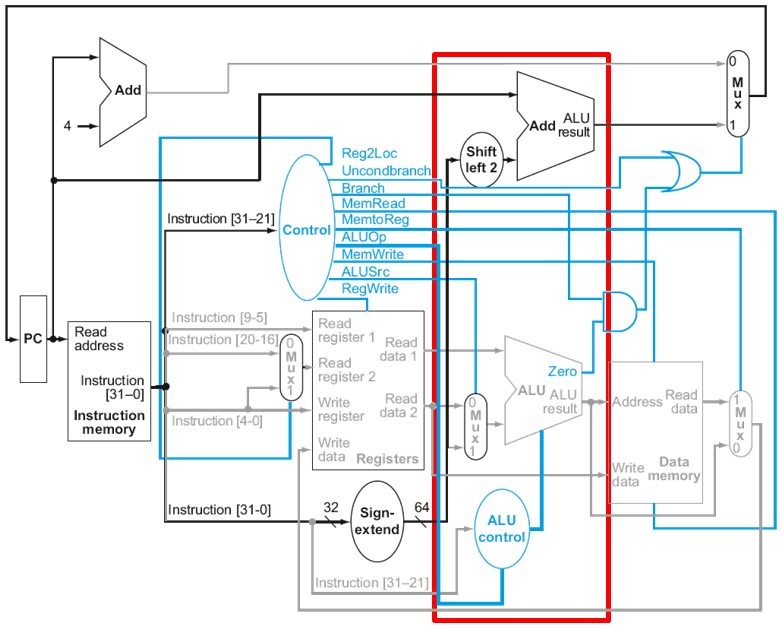
\includegraphics[width=4.75in]{../images/execute_stage.png}
	\end{center}
\end{figure} 

These five modules should be included in a new module called iExecute.  iExecute should consist of everything shown in the red box on Figure ~\ref{fig:execute_stage}. 

\section{Your Assignment}
I have provided a test bench, iExecute\_test.v.  Feel free to modify and improve it as you see fit.

You are to:
\begin{enumerate}
\item Complete the iExecute module and use the iExecute\_test to verify that you get the results that you expect.
\item Write up a lab report in \LaTeX\ following the lab format in \verb1LabN.tex1 and generate a pdf file.
\item Upload the pdf and all the Verilog files to Canvas.
\item If you finish early, you can probably predict what is next....integrate iExecute into datapath.v and get the first 3 stages working together properly.  Feel free to get started.
\end{enumerate} 